\documentclass[conference]{IEEEtran}
\IEEEoverridecommandlockouts
% The preceding line is only needed to identify funding in the first footnote. If that is unneeded, please comment it out.
\usepackage{cite}
\usepackage{amsmath,amssymb,amsfonts}
\usepackage{algorithmic}
\usepackage{graphicx}
\usepackage{textcomp}
\usepackage{xcolor}
\usepackage[utf8]{inputenc}
\def\BibTeX{{\rm B\kern-.05em{\sc i\kern-.025em b}\kern-.08em
    T\kern-.1667em\lower.7ex\hbox{E}\kern-.125emX}}
%For Listings:
\usepackage{listings}
\lstset{
  frame=single,
  language=C,
  basicstyle=\footnotesize,
}
\makeatletter
\def\lst@makecaption{%
  \def\@captype{table}%
  \@makecaption
}
\makeatother
\begin{document}

\title{Task-based Analysis of OpenMP and HPX}

\author{
\IEEEauthorblockN{Tobias Schiffmann}
\IEEEauthorblockA{
\textit{Universität Stuttgart}\\
Stuttgart, Germany \\
st169736@stud.uni-stuttgart.de}
}

\maketitle

\begin{abstract}
Task-based programming is used to parallelize irregular structures like recursive function calls.
A prominent examples for run time systems allowing to utilize tasks are OpenMP and HPX.
OpenMP is the de facto standard for shared memory parallel programming and in contrast to this HPX is a rather new run time system designed for task-based programming.

These two systems have not yet been compared concerning tasking performance.
To do so the Fibonacci, Merge Sort and a generic algorithm are implemented using both run time systems.

The performances of the executions are compared and some optimization ideas are evaluated.

It comes clear that both run time systems have structures they perform better with compared to the other system.
HPX has problems managing high amounts of small tasks in hierarchical structure, however it achieves better performance with bigger tasks and non hierarchical structures.
\end{abstract}

\begin{IEEEkeywords}
High Performance Computing, HPX, OpenMP, Task-based Parallelism
\end{IEEEkeywords}

\section{Introduction}
\cite{Ayguade.2009}
  - irregular and dynamic structures, eg while loops, dynamic inked list traversal and recursive calls
  - defining independent units of work which can be scheduled
    --> tasking
  - tasks can exploit irregular parallelism
  - mixing data and task parallelism improves the overall performance of an application (additional sources are provided)

\cite{Qawasmeh.2014}
  - two crucial issues should be managed by any task scheduler
    - data locality in terms of cache and load balancing


\section{Related Work}

\subsection{Tasking}
\label{subsec:Tasking}
  Having the task construct as mean to parallelize a program allows to utilize irregular parallelism.
  This type of parallelism utilizes irregular data structures, e.g. linked lists rather than arrays.
  Furthermore communication phases and the needed amount of communication cannot be identified in advance.
  This is also the case for the amount of computation.\cite{Chakrabarti.1993}
  Parallel execution of while loops or recursive function calls perform irregular parallelism for instance.
  Tasking explicitly specifies independent units of work which can be executed in parallel.
  This enables a more dynamic way of parallelization which can handle irregular parallelism.
  However, a disadvantage of this kind of parallelism is that it increases the complexity of a program and poor implementations can lead to an increased overhead.~\cite{Ayguade.2009}~\cite{LaGrone.2011} 
  
  The used runtime system for parallel execution plays a crucial role when it comes to the application's performance using tasking. 
  For example, as the tasking construct creates several tasks which will be executed by threads, the performance of an application relies on the thread scheduler of the runtime system.
  The authors of \cite{LaGrone.2011} discuss different aspects of a runtime system using the task construct.
  The efficiency of such depends on the data structures which store unfinished tasks, manage task switching and regulate task creation.
  Additionally, the data structures to organize task synchronization and manage the memory footprint of a task are also important.
  The ideal way of work of the thread scheduler, for example, is to maximize concurrency, load balancing and data locality.
  This can be achieved by different ways to manage queue storing all tasks ready to be executed.
  Furthermore, the scheduler can be \textit{depth-first} or \textit{breadth-first}.
  Breadth-first means that child tasks created by the parent task and put into the queue to be scheduled at any time.
  Whereas breadth-first schedulers switch to child tasks directly after their creation and execute them.
  This leads to a smaller number of tasks in the queue and less concurrency opportunities.
  However, the data reuse may increase depending on the running application.
 
 	
  The following subsections \ref{subsec:OpenMP} and \ref{subsec:HPX} introduce two runtime systems utilizing tasks.
  These will be compared in this work.


\subsection{Tasks in OpenMP}
\label{subsec:OpenMP}
  OpenMP includes the tasking model since version 3.0.
  Various directives for that purpose are being included since to specify and manage  tasks.
  However, OpenMP still differs between explicit and implicit tasks.
  Implicit tasks are created by parallel regions as side effect.
  The programmer does not need to specify or know about them.
  Explicit tasks on the other hand are defined by the programmer using the task directives.
  The simplest directive to define an explicit task is \texttt{omp task} and the enclosed code area is the task region.
  These are executed by any task in the current team whenever they are ready.~\cite{Ayguade.2009}~\cite{LaGrone.2011}

%MAYBE example implementation here - show the directives

  When a thread encounters a task directive the current data environment is captured.
  This environment and the block of code in the task region form the generated task.
  The variable scopes of a task region can be defined like in parallel regions.
  By adding the clauses \texttt{shared}, \texttt{private} or \texttt{firstprivate} to the task directive the declared variables are either shared among tasks or not.~\cite{Duran.2008}
  
  
  By default a thread is tied to a task as it begins to execute it.
  This means that this task is only allowed to be executed by one thread.
  However this thread can still execute other tasks in case it reaches task scheduling points and switches the execution to another task.
  The suspended task is put into the queue and has to wait until its tied thread is ready to continue its execution.
  This restriction can be avoided by defining the task \texttt{untied}.
  By doing so, load balancing is increased, but data locality is decreased.~\cite{Ayguade.2009}~\cite{LaGrone.2011}


  Tasking results in a more dynamic execution and might be unpredictable without explicit scheduling.
  For example the runtime system has either a depth- or breadth-first scheduler.
  Meaning that it either switches to the child task after creation or finishes the parent task first.
  The used OpenMP runtime system is responsible to decide.
  Explicit scheduling can be used to avoid this uncertainty.
  For instance, adding an \texttt{if}-clause to the task directive and evaluating it to false makes the encountering thread to suspend its current work and execute the child task immediately.
  Furthermore, explicit task scheduling is possible by using the \texttt{taskwait} and \texttt{barrier} directives.
  \texttt{taskwait} suspends the encountering task region and forces it to wait for all child tasks to complete.
  Additionally \texttt{taskgroup} defines a task region which will be executed and at the end the current task has to wait for all its child and their descendants.~\cite{Qawasmeh.2014}~\cite{Furlinger.2009}


\subsection{HPX}
\label{subsec:HPX}
\subsubsection{HPX}
  %1\cite{Kaiser.2014}
  %2\cite{Kaiser.2009}	  
  
  HPX aims to resolve problems in scalabilitiy, resource management and even further ones which may raise and increase by moving from Peta- to Exascale systems.
  It focuses on parallel and distributed development independent of the system's scale.
  This is done by providing a general purpose C++ runtime system with an innovative design.
  It is described by the authors of \cite{Kaiser.2014} as a mixture of lightweight synchronization, global system-wide address space and fine grain parallelism.
  Message driven computation can be achieved with a small amount of effort.
  A remote execution has the same semantics as a local one and can thereby be done implicitly.
  Furthermore, it offers the programmer explicit support for accelerators such as general purpose graphical processing units.~\cite{Kaiser.2014}
  
  
  A new model of parallel execution is introduced to enable all of this features --- called \textit{Parallex}.
  HPX is the runtime system supporting this new model.
  It consists of components which can be seen in figure \ref{fig:HPXcomp}.
  Additionally, it shows the current architecture of HPX and how the following ParalleX components are included.~\cite{Kaiser.2009}\\
  \textbf{Parcel Subsystem} encapsulates method calls into parcels.
  These contain the global address of the object whose method is called and the necessary arguments.
  Parcels are communicated via localities which are placed on each node and can be seen as parcel interfaces.
  Localities thereby represent single nodes in the execution network.
  The parcel subsystem is especially useful when it comes to remote method calls as it eases the work transfer between localities.\\
  \textbf{Active Global Address Space (AGAS)} includes all localities the current application is using.
  Global identifiers ease to locate objects in the network.
  Having this global address space furthermore allows to move objects across localities without changing its address.\\  
  \textbf{Instrumentation and Adaptivity} includes several performance countering and monitoring tools.
  They might be helpful when debugging or analyzing the program and offer insights without using additional tools.\\
  \textbf{Threading Subsystem} uses a work-queue based execution strategy to schedule HPX threads.
  These are either created locally or the threading subsystem converts parcels on receive into HPX threads.
  In contrast to other systems the ParalleX model maps \(m\) internal threads instead of just 1 onto \(n\) kernel threads.
  This allows ParalleX to switch between threads without the need of kernel calls and their context switch overhead.\\  
  \textbf{Local Control Objects (LCO)} are used for scheduling and abstract mechanism used to do so.
  For example, \textit{futures} are proxies for results not yet known and can only be accessed after the result is available.
  In case the future is accessed earlier, the thread doing so is suspended.
  Additional to special objects such as futures, HPX also offers traditional concurrency control mechanisms, for instance mutexes and semaphores.
\begin{figure}[htbp]
	\centering
	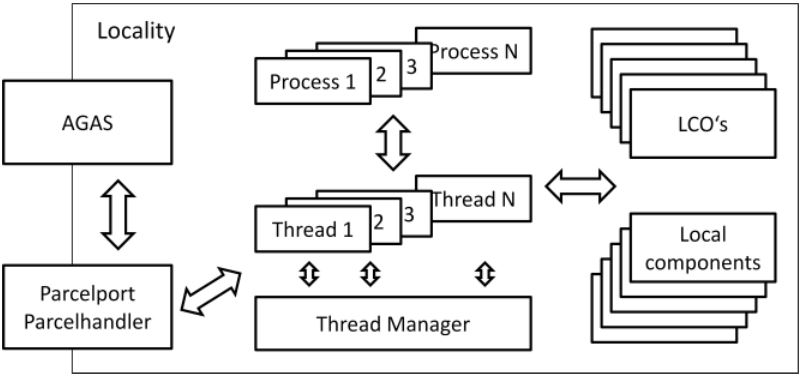
\includegraphics[width=0.45\textwidth]{figures/parallexArchitecture.JPG}
	\caption{ParalleX Components Implemented in HPX~\cite{Kaiser.2009}}
	\label{fig:HPXcomp}
\end{figure}
  	
	
\subsubsection{Tasks in HPX}
  \label{subsubsec:TasksHPX}
  Various program models increase their efforts on tasking in recent years and increase the possibilities in local parallelism.
  However, in contrast to the other program models, HPX offers a way for homogeneous execution of local and remote operations.
  This is achieved by using the task model combined with a so called \textit{Active Global Address Space}.
  As all nodes of an application share a common address space, objects and tasks can be migrated across nodes.
  Instead of moving the data to nodes the tasks can be moved to the data, which allows faster communication as the instructions are often smaller in size than the actual data.
  Furthermore the migration can be done without changing the global address as all nodes share the address space.
  Additional work is saved due to this fact.~\cite{Kaiser.2014}
  
  Another advantage of HPX which also makes it convenient to C++/C programmers is that it uses the same tasking methods as the C++ standard.
  No new semantic or syntax is used.
  However, the actual standard is extended to support remote operations.
  To use tasking in HPX, tasks have to be defined by \texttt{async} and \texttt{future}.
  \texttt{async} launches a task asynchronously.
  \texttt{future<T>} represents a value of type \texttt{T} which will be available in the future, when the execution of a task finishes.
  It acts as a placeholder of a result not known yet and when created spawns a new HPX-Thread which is placed on the thread queue.
  In case another thread wants to access a future it is blocked and has to wait until the value of the future is available.
  Using \texttt{get()} is an explicit option for the programmer to let the thread wait for the future.~\cite{Kaiser.2014}~\cite{TheSTEARGroup.2020}
  
  
  The HPX thread scheduling system uses lightweight threads which allow faster context switches and smaller stacks.
  Task migration is therefore more efficient as less data has to be moved.
  Furthermore, it is designed to handle millions of tasks efficiently.
  In \cite{Kaiser.2014} HPX tasks are compared to OpenMP tasks for their GFLOPS on various numbers of cores.
  However the HTTS benchmark is used which uses no-op tasks and can therefore only compare the thread scheduling performance without actual workload.
  One reason why HPX performed better in the HTTS benchmark is that it uses constraint based synchronization instead of global barriers, like in OpenMP.
  For example, OpenMP uses implicit barriers at the end of each loop.
  In contrast to that HPX allows to execute the code following the loop in case no data dependencies are given.
  
     
\subsection{Benchmark Algorithms}
\label{subsec:BOTS}
  The authors of \cite{Duran.2009} introduce a benchmark suite to test the impact of different implementation decisions using OpenMP tasks.
  The benchmark suite is called \textit{Barcelona OpenMP Task Suite (BOTS)} and includes nine benchmarks:\\
    \textbf{Alignment} is an algorithm aligning protein sequences against every other sequence.\\
    \textbf{Fourier Transformation} tries to approximate a periodic function by several subfunctions.\\
    \textbf{Fibonacci} calculates the \(n^{th}\) number of the Fibonacci sequence.\\
    \textbf{Floorplan} computes the optimal floorplan distribution of a number of cells.\\
    \textbf{Health} simulates the Colombian Health Care System.\\
    \textbf{N Queens} tries to find placements of \(n\) queens on a chessboard under special condition.\\
    \textbf{Sort} is a special kind of parallel merge sort execution.\\
    \textbf{SparseLU} calculates a LU matrix factorization over sparse matrices.\\
    \textbf{Strassen} hierarchically decomposes a matrix for multiplication of large dense matrices.\\
  The suite offers different versions of each benchmark, e.g. a version of Fibonacci using a cut-off to avoid an high amount of tasks.
 
 
\subsection{hpxMP}
  A rather new approach is \textit{hpxMP}.
  It's an implementation of the OpenMP standard using an underlying hpx system and introduced in \cite{hpxMP.2019}.
  The motivation of this approach is to ease the migration from OpenMP to Asynchronous Many-Task (AMT) systems.
  AMT as a new parallel programming paradigm utilizes fine grained tasks to distribute the workload across multiple node.
  It is similar to the well known \textit{MPI+X} approach in which the Message Passing Interface (MPI) is used together with OpenMP for example.
  However, for certain applications MPI+X offers less scalability and parallel efficiency compared to AMTs, for instance in \cite{Dai.11172019}.
  HPX as an example for an AMT might also be more convenient as it follows the newest C++ standard and therefore has a more flatten learning curve for C++ programmers.
  Another advantage of hpxMP might have in contrast to MPI+X is that it uses HPX lightweight threads instead of system threads.
  They are briefly explained in \ref{subsubsec:TasksHPX}.
  
  \begin{figure}[htbp]
	\centering
	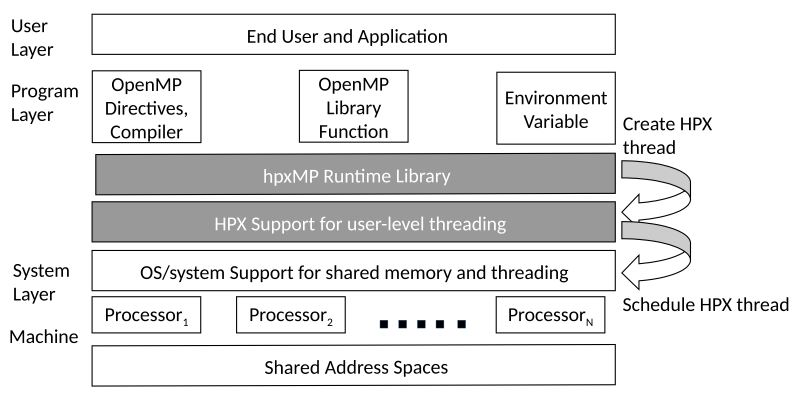
\includegraphics[width=0.48\textwidth]{figures/hpxMP.JPG}
	\caption{Adaption of an OpenMP Application to use hpxMP~\cite{hpxMP.2019}}
	\label{fig:hpxMP}
  \end{figure}
  
  Figure \ref{fig:hpxMP} shows how hpxMP can be used to run OpenMP applications.
  The application is compiled with OpenMP flags, but linked against the hpxMP runtime library being the first grey layer in the figure.
  Instead of calling the OpenMP functions, equivalent hpxMP functions are called.
  These redirect the calls to appropriate functions of the underlying HPX system being the next grey layer in the figure.
  This system allows to execute OpenMP applications using HPX according to the OpenMP standard.
  
  The authors of \cite{Zhang.2192020} furthermore extended hpxMP with further task features of the OpenMP 5.0 standard.
  Additionally, they compared the new hpxMP system with different OpenMP implementations.
  Among other benchmarks, they used the BOTS merge sort algorithm.
  The cut off option is used to decrease the number of tasks spawned.
  The results show that hpxMP can already reach similar or better performance results for larger input sizes.
  This is due to the fact that joining a large number of tasks after a parallel region produce less overhead using HPX threads.
  Compared to conventional operating system threads HPX threads are lightweight and need less effort when joining.
  However for smaller input sizes hpxMP reaches slower performance.
  The authors explain this by the overhead which is introduced by the HPX scheduler.
  Conventional threads spawned by OpenMP may not be suspended and therefore need to be scheduled less often.
  

\section{Implementation \& Design}
\label{sec:implem}
  For this paper the Fibonacci and the Sort algorithm from BOTS are chosen to be implemented, as introduced in subsection \ref{subsec:BOTS}.
  Additionally, a generic algorithm is implemented.
  All three are implemented using OpenMP, HPX and in a sequential way.
  
  \paragraph{Fibonacci}
  The algorithm can spawn a high amount of tasks with small workload.
  The workload of forking and joining new threads might have the biggest impact when it comes to performance.
  
  The implementation is done without cut offs for the HPX and OpenMP versions.
  This means that every recursive call of the Fibonacci function creates a new task.
  \begin{lstlisting}[
  caption=Fibonacci OpenMP Implementation,
  label=lst1:fibOMP,
]
long long fibonacci(long long input) {
    if (input < 2 ) return input;
    long long x, y;
    #pragma omp task shared(x) firstprivate(input)
    x = fibonacci(input - 1);
    #pragma omp task shared(y) firstprivate(input)
    y = fibonacci(input - 2);
    #pragma omp taskwait
    return x + y;
}
\end{lstlisting}
  Listing \ref{lst1:fibOMP} shows a first implementation of the Fibonacci algorithm using OpenMP.
  It shows which directives are used.
  As explained in subsection \ref{subsec:OpenMP}, the \texttt{\#pragma omp task} directive creates a new task which may be executed.
  Using the \texttt{shared} and \texttt{firstprivate} clauses adjusts the variable scopes so that each task has its own instance of the parameter input.
  Variables \texttt{x} and \texttt{y} are shared which means no new instance is created.
  At the end the \texttt{\#pragma omp taskwait} directive tells the function to wait until all the child tasks finished their execution.
  
\begin{lstlisting}[
  caption=Fibonacci HPX Implementation,
  label=lst1:fibHPX,
]
long long fibonacci(long long input) {
  if (input < 2) return input;
  hpx::future<long long> n1 =
      hpx::async(fibonacci, input - 1);
  long long n2 = fibonacci(input - 2);
  return n1.get() + n2;
}
\end{lstlisting}
  The HPX implementation of the Fibonacci algorithm can be seen in listing \ref{lst1:fibHPX}.
  In contrast to OpenMP, HPX works with futures to abstract results of function calls.
  Calling a function with \texttt{hpx::async} creates a task and immediately returns a future to continue the execution.
  Calling \texttt{get} on a future suspends the current thread until this future is returned.
\begin{figure}[htbp]
	\centering
	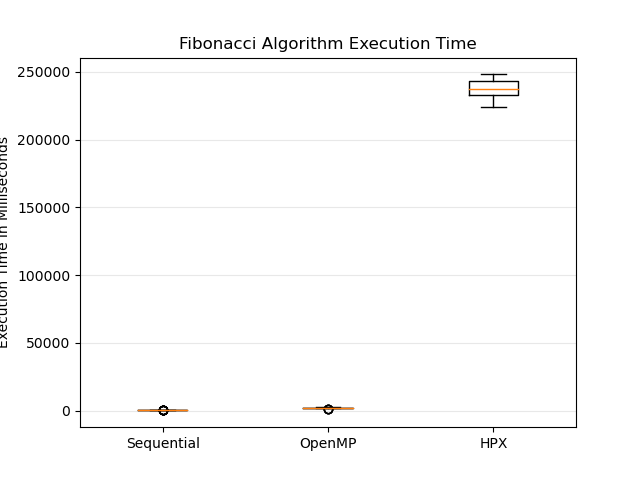
\includegraphics[width=0.45\textwidth]{figures/fib_NoOp.png}
	\caption{Execution times of the Fibonacci algorithm}
	\label{fig:fib_NoOp}
\end{figure}

Figure \ref{fig:fib_NoOp} shows boxplots of 100 runs of the 22\textsuperscript{nd} Fibonacci number.
It illustrates the execution times of the sequential, OpenMP and HPX version.
The sequential and OpenMP implementation need the fewest time to complete, whereas the HPX version takes a lot more time.
This is due to the fact that HPX threads may be suspended in contrast to threads in OpenMP resulting in the HPX implementation having a bigger scheduling overhead.
Although the joining process at the end of a task region produces less overhead in HPX.
  \\
 
  \paragraph{Merge Sort}
  The Sort algorithm of BOTS is slightly adjusted to a normal merge sort.
  It is a suitable use case, easy to implement and can also spawn a high number of tasks.
  Also in case of merge sort no cut off is implemented.
  \begin{figure}[htbp]
	\centering
	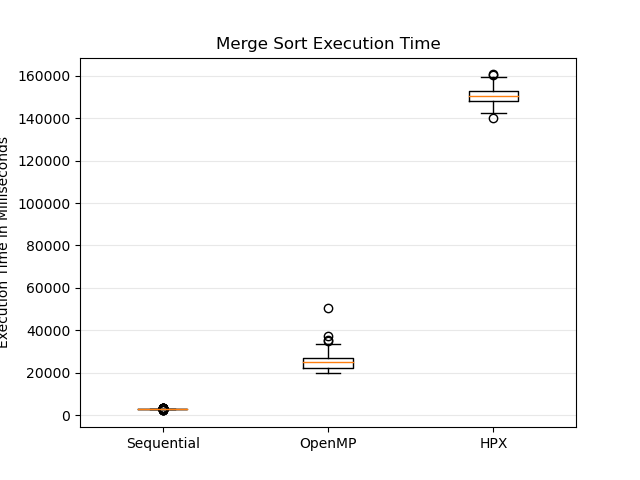
\includegraphics[width=0.45\textwidth]{figures/sort_NoOp.png}
	\caption{Execution times of Merge Sort}
	\label{fig:sort_NoOp}
  \end{figure}
  The measurements of figure \ref{fig:sort_NoOp} are created on environment three and show the average of 100 runs.
  The merge sort is run on 10.000 random elements which are created in a deterministic way.
  Similar to Fibonacci, merge sort also creates a lot of tasks and HPX shows the slowest execution time.
  Sequential has the shortest average time and the OpenMP average times differ more significantly this time compared to the Fibonacci example. 
  \\
  
  \paragraph{Generic Algorithm}
  The aim of this algorithm is to enable task size adjustment and allow to define the number of tasks.
  
  The algorithm uses two vectors which sizes are defined at the building process.
  First of all one vector is filled by randomized floating point numbers.
  To compare each run a deterministic seed for the random numbers is chosen.
  In each turn the element of a vector is equal to a calculation on the element of the other vector.
  The sinus function is calculated on the element before it is multiplied by ten and adjusted to an absolute value.
  This turns are repeated a defined number of times.
  After the last turn is executed, all elements of the last calculated vector are summed up.
  
  The task size can be adapted by parameters and defines how many vector elements are calculated by a task.
  The task size furthermore defines how many tasks are used per run.
  This number is equal to the vector size divided by the task size.
  As each turn depends on the execution of the previous turn, the number of dependencies can be increased by using more tasks per turn.
\begin{figure}[htbp]
	\centering
	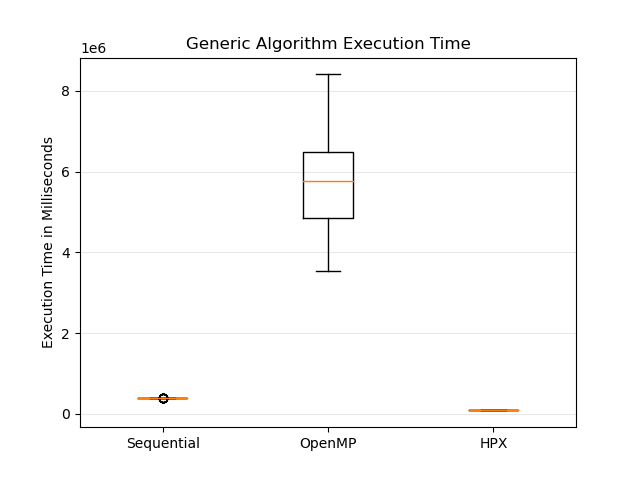
\includegraphics[width=0.45\textwidth]{figures/generic_NoOp.png}
	\caption{Execution times of the generic algorithm}
	\label{fig:gen_NoOp}
\end{figure}

Figure \ref{fig:gen_NoOp} shows the measured execution times for the generic algorithm in his three versions.
Again these are the average values of 100 runs on the system of environment three.
20 turns are made with a task size of 20 and the array size is 1,048,576.
It can be seen that the range of OpenMP times is quite big compared to the sequential and HPX version.
Additionally, the OpenMP version takes the longest time to complete the execution whereas HPX is the fastest of these three. 


\section{Environment}
  The code is executed on different systems which differ in hardware configuration.
  This might show different behavior of the implementations in different contexts.

The hardware specifications of the three environments can be seen in table \ref{tab:hardEnv}.
Environment 1 has has an Intel Xeon Phi 7210 processor with 64 cores and the available memory is about 92 GB.
Environment 2 contains about 124 GB and an AMD EPYC 7551P processor which has a number of cores equal to 32.
The third environment owns a 64 cored AMD EPYC 7742 processor. The available memory is quite small compared to the other environments, but sufficient.
It has a size of about 3.8 GB.
\begin{table}
\centering
\caption{Hardware Specification of the Environments}
\begin{tabular}[h]{l c c c}
% 1: argon-knl, 2: argon-epyc, 3: IPVS-epyc
 & Environment 1 & Environment 2 & Environment 3  \\\hline
CPU & Intel Xeon Phi 7210 & AMD EPYC 7551P & AMD EPYC 7742 \\
RAM & $\sim 92$ GB & $\sim 124$ GB & $\sim 3.8$ GB \\
Cores & 64 & 32 & 64 \\\hline
\end{tabular}
\label{tab:hardEnv}
\end{table}

The software specifications of the environments can be seen in table \ref{tab:softEnv}.
On all systems the same software versions are used and contain \texttt{GCC}, \texttt{HPX}, \texttt{Boost} and \texttt{OpenMP}.
HPX and Boost are installed and build by using Spack~\cite{Spack.2020} which is a package management tool.
\begin{table}
\centering
\caption{Software Specification of the Environments}
\begin{tabular}[h]{l c c}
\centering
 & Environment 1 & Options\\\hline
Compiler & GCC 9.2.0 & \\
HPX Version & 1.4.0 & cxxstd=14 networking=none  \\
Boost Version & 1.70.0 & cxxstd=14 \\
OpenMP Version & 4.5 & \\\hline
\end{tabular}
\label{tab:softEnv}
\end{table}

\section{Results \& Discussion}

The results of the three algorithms in this section are created on environment three.
They are illustrated using boxplots showing the execution time of 100 runs.


\paragraph{Fibonacci}
\begin{figure}[htbp]
	\centering
	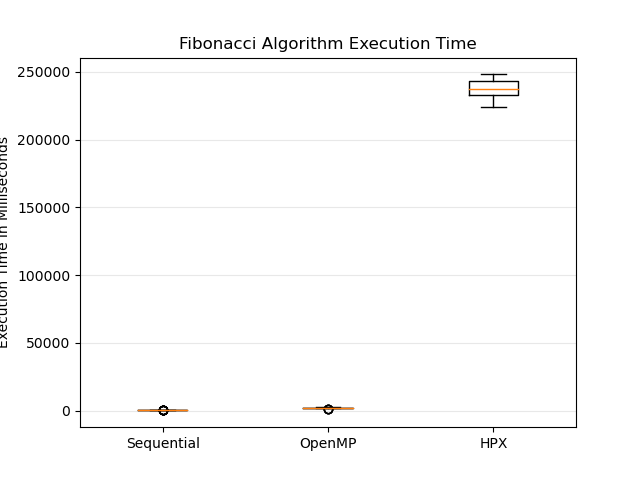
\includegraphics[width=0.45\textwidth]{figures/fib_NoOp.png}
	\caption{Execution Times of Fibonacci Algorithm (Environment 3, 64 Threads)}
	\label{fig:fib_NoOp}
\end{figure}

Figure \ref{fig:fib_NoOp} shows the execution time of the 22\textsuperscript{nd} Fibonacci number.
It illustrates the times of the sequential, OpenMP and HPX version.
The sequential and OpenMP implementation need the fewest time to complete, whereas the HPX version takes a lot more time.

\paragraph{Merge Sort}
  \begin{figure}[htbp]
	\centering
	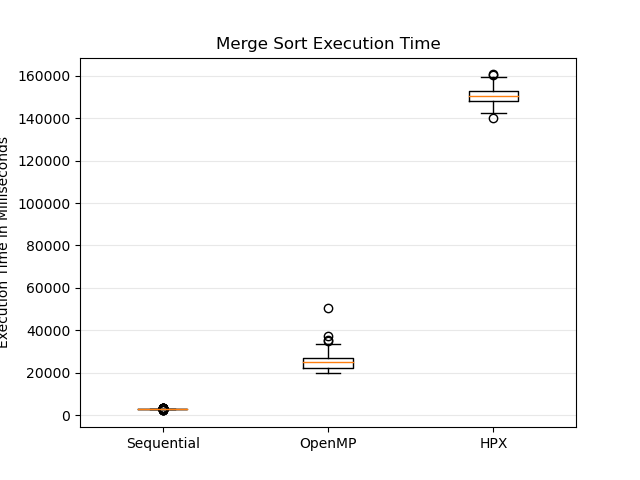
\includegraphics[width=0.45\textwidth]{figures/sort_NoOp.png}
	\caption{Execution Times of Merge Sort (Environment 3, 64 Threads)}
	\label{fig:sort_NoOp}
  \end{figure}
  The measurements of figure \ref{fig:sort_NoOp} show the execution times of Merge Sort.
  The algorithm is run on 10.000 random elements which are created in a deterministic way.
  Similar to Fibonacci, merge sort also creates a lot of tasks and HPX shows the slowest execution time.
  Sequential has the shortest average time and the OpenMP average times differ more significantly this time compared to the Fibonacci example.
  
\paragraph{Generic Algorithm}
  \begin{figure}[htbp]
	\centering
	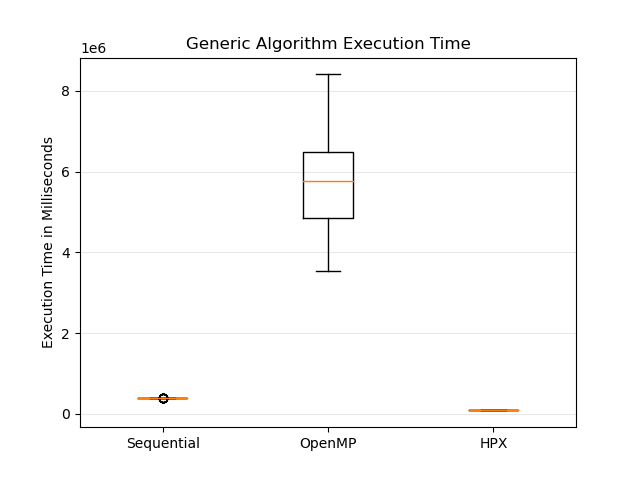
\includegraphics[width=0.45\textwidth]{figures/generic_NoOp.png}
	\caption{Execution Times of Generic Algorithm (Environment 3, 64 Threads)}
	\label{fig:gen_NoOp}
\end{figure}
Figure \ref{fig:gen_NoOp} shows the measured execution times for the generic algorithm in his three versions.
20 turns are made with a task size of 20 and the array size is 1,048,576.
It can be seen that the range of OpenMP times is quite big compared to the sequential and HPX version.
Additionally, the OpenMP version takes the longest time to complete the execution whereas HPX is the fastest of these three. 

\subsection{Discussion}
It can be seen that HPX has some issues keeping up with the sequential and OpenMP implementation of Fibonacci and Merge Sort.
Both algorithms spawn a lot of tasks in hierarchical structure.
This means each task, except of the root task, has a parent task.
This parent task has to suspend its execution until its child tasks finished their execution.
In contrast to threads in OpenMP HPX threads may be suspended which results in scheduling tasks occurring more often.
This leads to a bigger scheduling workload for HPX.

The generic algorithm however uses a different structure as it spawns various tasks for an array which need to be finished before spawning the next tasks for the next turn.
In this concept HPX can use its strength of lightweight threads.
These fork and join faster and with less work to do.



\section{Optimization}
\label{sec:Opt}
\subsection{Fibonacci - Cutoff}
  One possible optimization used in the BOTS benchmarks is implementing a cutoff option.
  This can be achieved by using an if clause which is provided by the task directive as it is described in \cite{MKlemm.2018}.
  In case this clause evaluates to false no task will be spawned and the execution continues with the function call in a normal sequential way.
  The cutoff value is used to specify at which level the tasking spawning has to be stopped.
  A level parameter is added to the Fibonacci function and increased every recursive call.
  In case the level parameter is equal or greater than the cutoff value, the Fibonacci algorithm will be continued sequentially without spawning tasks. 
  Table \ref{tab:cutoff} shows the results without a cutoff and with a cutoff level equal to eight calculating the Fibonacci number of 22.
  The mean values of 100 runs are \(2057.34\) ms and \(394.87\) ms for OpenMP without and with a cutoff.
The average measurements for HPX are \(237491.49\) ms without and \(5267.67\) ms with cutoff.
It can be seen that the HPX implementation benefits more by the cutoff.
HPX speeds up by a ratio of approximately \(45\) and the OpenMP implementation speeds up only by \(5\).

\begin{table}
\centering
\caption{Execution times of the Fibonacci algorithm with cutoffs in milliseconds}
\begin{tabular}[h]{|l|c|c|}
\hline
 & With Cutoff & Without Cutoff \\\hline
OpenMP & \(2057.34\) ms & \(394.87\) ms \\\hline
HPX & \(237491.49\) ms & \(5267.67\) ms \\\hline
\end{tabular}
\label{tab:cutoff}
\end{table}

\subsection{OpenMP - untied / tied Tasks}
  Another optimization approach might be to see if there is a difference in using tied or untied tasks.
  Untied tasks improve the load balancing as each free thread can start executing a task which is ready to be executed.
  The disadvantage of untied tasks is that the data is not always available locally.
  This means in case a thread wants to execute a ready task which is not created by it, the data and context has to be transferred to new execution location.
  
\begin{figure}[h]
	\centering
	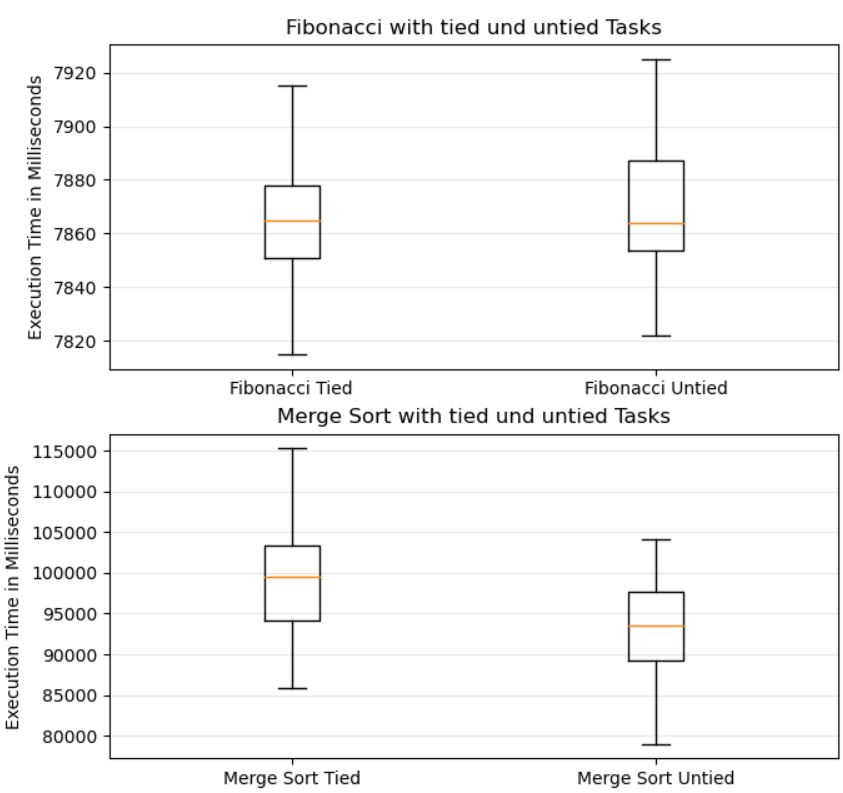
\includegraphics[width=0.45\textwidth]{figures/tied.JPG}
	\caption{Execution times of Fibonacci and Merge Sort with tied and untied Tasks in OpenMP (Environment 1, 256 Threads)}
	\label{fig:tied}
\end{figure}

  This experiment is run on environment 1 calculating again the Fibonacci number of 22.
  As figure \ref{fig:tied} shows there is no significant difference in execution time for both algorithms.
  Using tied or united tasks may only have minor impacts.
  As already mentioned this is due to the trade of of data locality and load balancing. 
  
\subsection{HPX - Fibonacci Dataflow}
HPX provides further LCOs than just futures.
Another object which might be useful is the \textit{dataflow} object.
It is an object which is used to define dependencies in functions easily.
Dataflows take a function and its parameters when initialized and call the function when all of its parameters are available. 
This might be the case for example if parameters are returned by futures.
However, it is also possible to concatenate dataflow objects to create a dependent hierarchy.~\cite{TheSTEARGroup.2020}

This experiment compares the HPX Fibonacci implementation using two futures with an implementation utilizing dataflows and another Fibonacci implementation using \texttt{when\_all}.
The last approach follows the same concept as the dataflow implementation, but works without this object type.
\texttt{when\_all} takes futures as parameters and starts executing when the values of all futures are available.
For this implementation the example code of HPX is taken as reference.~\cite{HPXGitHub.2020}
The idea is to utilize the dataflow principle to avoid blocked tasks and increase the scheduling overhead.

\begin{figure}[h]
	\centering
	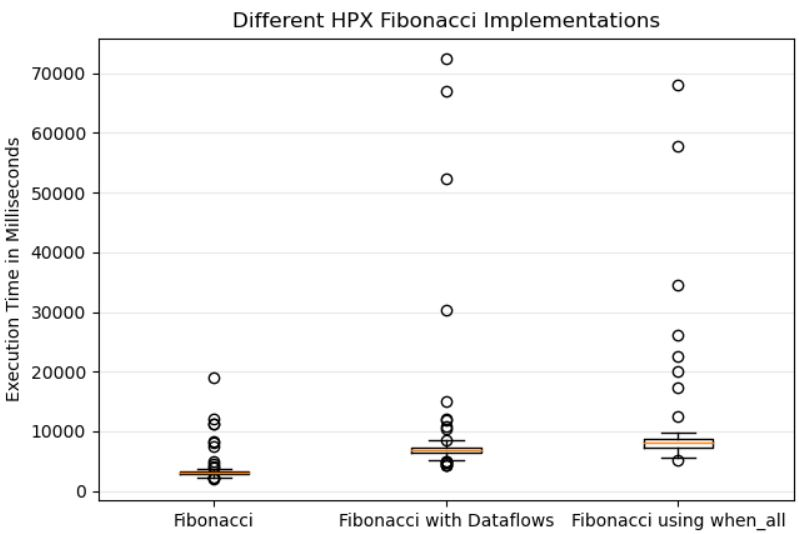
\includegraphics[width=0.45\textwidth]{figures/fibDataflow.JPG}
	\caption{Execution Times of Fibonacci using HPX and different Dataflow Constructs (Environment 3, 64 Threads)}
	\label{fig:fib_dataflow}
\end{figure}

The average execution times of 100 runs on environment 3 for the 22\textsuperscript{nd} Fibonacci number's calculation are illustrated in figure \ref{fig:fib_dataflow}.
It can be seen that the normal Fibonacci implementation has the shortest execution times of these three.
This means that the dataflow principle cannot help avoiding scheduling overhead for HPX implementations.
Instead it produces additional overhead.


\subsection{HPX - Thread Scheduling Policies}
 The authors of \cite{hpxMP.2019} and \cite{TheSTEARGroup.2020} state different thread scheduling policies in HPX.
 However, not all of them are available at the HPX version used.
 Therefore only the policies used are explained.
 The experiment is run on environment 2.\\
 \textbf{local-priority} gives each operating system (OS) thread one queue they can pull their work from.
 Furthermore a high and low priority queue are created which is accessible by each OS thread.
 Work from these queues is only pulled in case the dedicated OS thread queue is empty.
 In doing so the high priority queue's work is taken first.
 Additionally, the local-priority policy is available in first-in-first-out (fifo) and last-in-first-out (lifo) version.\\
 \textbf{local} only maintains one queue per OS thread the work is put to and pulled from.\\
 \textbf{abp-priority} is similar to the local-priority policy.
 There are also a global high priority and low priority queue.
 However all OS threads own a double ended lock free queue.
 Elements can be added and removed on both sides of this type of queue.
 Furthermore the abp-priority policy can also be used in fifo and lifo version.\\
 \textbf{static} has one queue per OS thread and tasks are distributed by round robin.
 In this policy no work stealing is available.\\
 \textbf{static-priority} is similar to local-priority as there are queues for each OS thread, high priority queues and low priority queues which can be accessed globally.
 In contrast to the local-priority policy the tasks are distributed by round robin and no work stealing is available.

\begin{figure}[h]
	\centering
	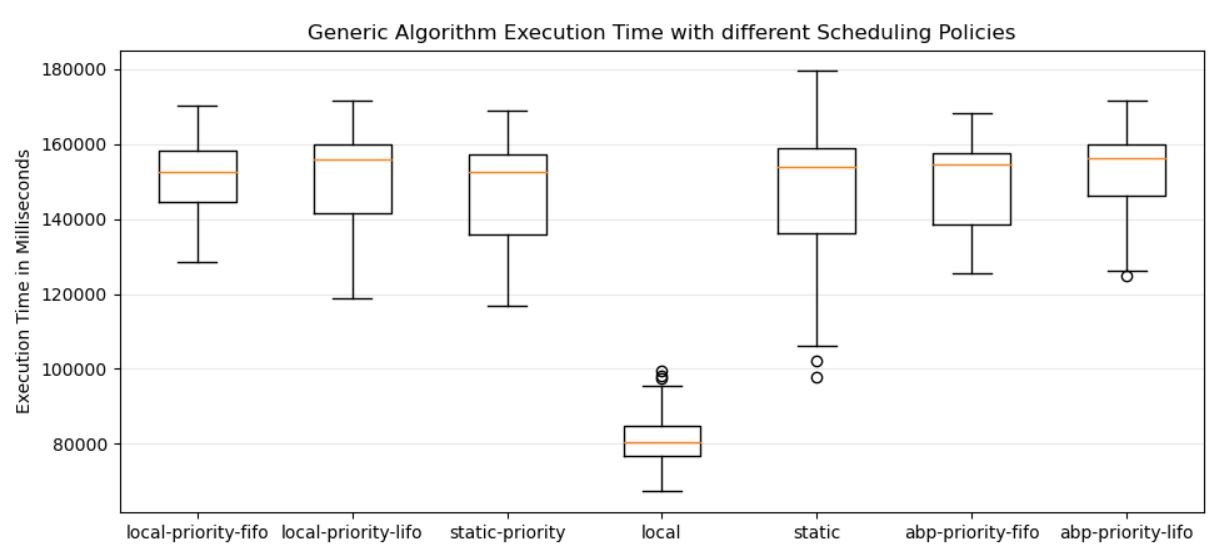
\includegraphics[width=0.45\textwidth]{figures/genSchedule.JPG}
	\caption{Execution Times of Generic Algorithm using different Scheduling Policies(Environment 2, 64 Threads)}
	\label{fig:gen_Schedule}
\end{figure}
\begin{figure}[h]
	\centering
	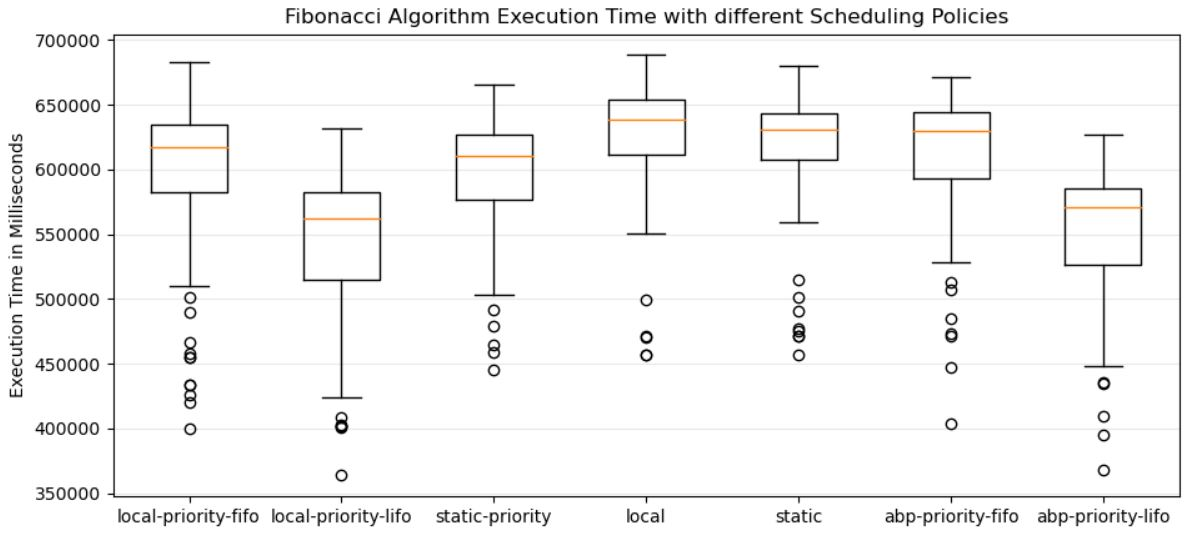
\includegraphics[width=0.45\textwidth]{figures/fibSchedule.JPG}
	\caption{Execution Times of Fibonacci Algorithm using different Scheduling Policies (Environment 2, 64 Threads)}
	\label{fig:fib_Schedule}
\end{figure}
\begin{figure}[h]
	\centering
	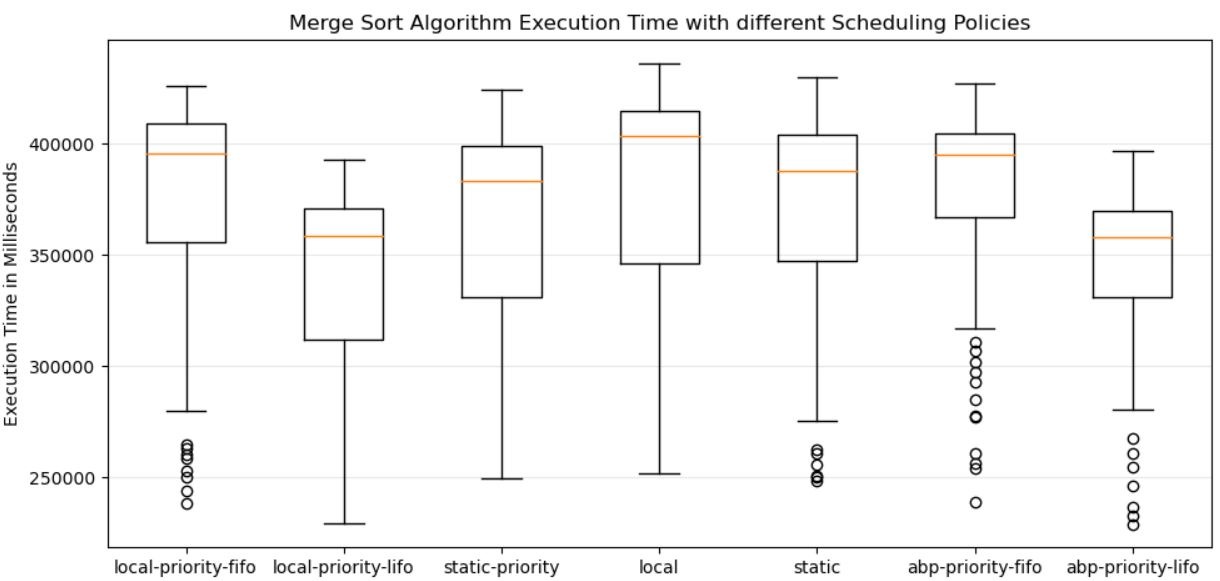
\includegraphics[width=0.45\textwidth]{figures/sortSchedule.JPG}
	\caption{Execution Times of Merge Sort Algorithm using different Scheduling Policies (Environment 2, 64 Threads)}
	\label{fig:sort_Schedule}
\end{figure}

The figures show the execution time of the three implemented algorithms with the previously explained thread scheduling policies.
The parameters are the same as stated in section \ref{sec:implem}.
Figure \ref{fig:gen_Schedule} is a boxplot diagram of the generic algorithm, figure \ref{fig:fib_Schedule} shows the execution times of the Fibonacci algorithm and figure \ref{fig:sort_Schedule} illustrates the execution times of Merge Sort.
It can be seen that the local policy accelerates the generic algorithm execution significantly compared to the other policies.
This may be because it produces little overhead as it does not have to maintain priority queues.
The significant difference to the static scheduling policy is that, when using the local policy, tasks are not distributed via round robin and task stealing is allowed.
These facts may lead to a better load balancing although the task size does not vary much.
The other two algorithms show no significant different in the policies.
However a trend can be seen as the mean values of the lifo policies show a shorter execution time in all cases.
This may be due to the fact that Fibonacci and Merge Sort create a task hierarchy in which the early created tasks are suspended till the end.

\subsection{Generic Algorithm - Number of Tasks}
For a better comparison of the three algorithms, various task sizes might be used.
The generic algorithm allows to adjust task sizes by parameters.
The second environment is taken for this test run in which tasks sizes ranging from 10 elements to 500 elements per task in steps of 10.
The total number of elements in the arrays \(1,048,576\) and the arrays are computed 50 times.
\begin{figure}[h]
	\centering
	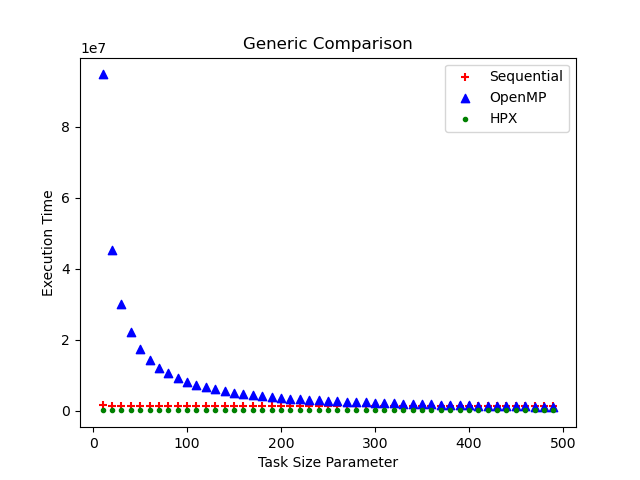
\includegraphics[width=0.45\textwidth]{figures/genericComp.png}
	\caption{Execution Times of Generic Algorithm with various Task Sizes (Environment 2, 64 Threads)}
	\label{fig:genComp}
\end{figure}

\begin{figure}[h]
	\centering
	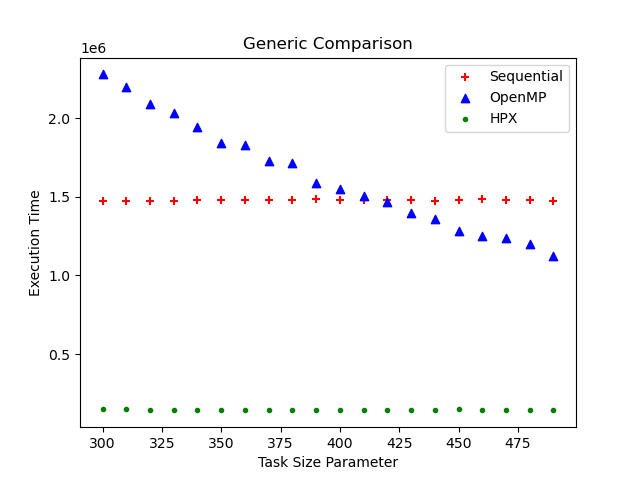
\includegraphics[width=0.45\textwidth]{figures/genericCompLast.png}
	\caption{Execution Times of Generic Algorithm with biggest Task Sizes (Environment 2, 64 Threads)}
	\label{fig:genComp_Last}
\end{figure}

Figure \ref{fig:genComp} illustrates the execution time for all three implementations.
The mean value of 50 measurements is taken.
It can be seen that the sequential and HPX implementation are quite constant.
In contrast, OpenMP takes more time when the task size is rather small and reaches the execution time of the sequential version at a task size of $\sim $410.
If the task size is bigger OpenMP takes less time compared to the sequential implementation.
However, it cannot reach the times of the HPX implementation.
Figure \ref{fig:genComp_Last} shows the same data however only the task sizes greater and equal to 300.
Especially, the trends of OpenMP and the sequential version can be seen in detail.
Important to mention is that changing the task size in the generic algorithm does not increase the overall workload.
This can be seen at the sequential implementation's constant graph.
Changing the task size does only increase or decrease the tasks which are created.
In contrast to the Fibonacci algorithm and Merge Sort, the generic algorithm does not create hierarchical dependencies.
Task synchronization is done when all elements of an array are calculated.
HPX benefits from that structure as the lightweight threads used produce less overhead when forking and joining.
The scheduling overhead is smaller than the benefit from the parallel execution and therefore HPX becomes faster than the sequential implementation.
The joining and forking overhead can be seen in the execution times of OpenMP.
OpenMP does have operating system threads and therefore produces more overhead having bigger amounts of tasks.
However, reaching a certain task size OpenMP also takes less time than the sequential execution of the generic algorithm.


\subsection{Generic Algorithm - Task Sizes}
\label{subsec:genAlgo}
As the previous example of the generic algorithm does only increase the amount of tasks used and not the overall workload, another approach is also implemented.
In this experiment the generic algorithm is adjusted to produce a squared workload per array element.
The workload can be adjusted by a parameter and varies in this experiment.
In contrast to the experiments before, each task does only contain one element.
This setup does allow to have a constant number of tasks with an option to increase or decrease the task size and overall workload.
In each task the elements value is multiplied a defined amount of times.
The parameter for defining this size is squared, which means that if the parameter is equal to 3 the element of the array is multiplied 9 times.
Each time the value is multiplied by the number of that multiply calculation.
In the example before first value will be multiplied by 1, then by 2, 3 and so on until it is multiplied by 9 in the last calculation.
The sinus function is then applied on the results and all of them are summed up and copied to the next array.
This principle is illustrated in \ref{fig:genMatrix_algo}.
\begin{figure}[h]
	\centering
	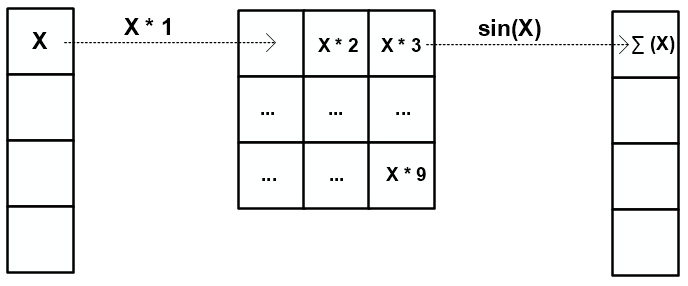
\includegraphics[width=0.45\textwidth]{figures/genericMatrix_algo.png}
	\caption{Principle of Generic Matrix Algorithm}
	\label{fig:genMatrix_algo}
\end{figure}

This experiment is also run on environment four having the same array size as the experiment before.
The number of calculations starts with 1x1 and increases by 2 in each dimension.
The biggest task size reached is 21x21.
For the HPX version the local thread scheduling policy is used.
\begin{figure}[h]
	\centering
	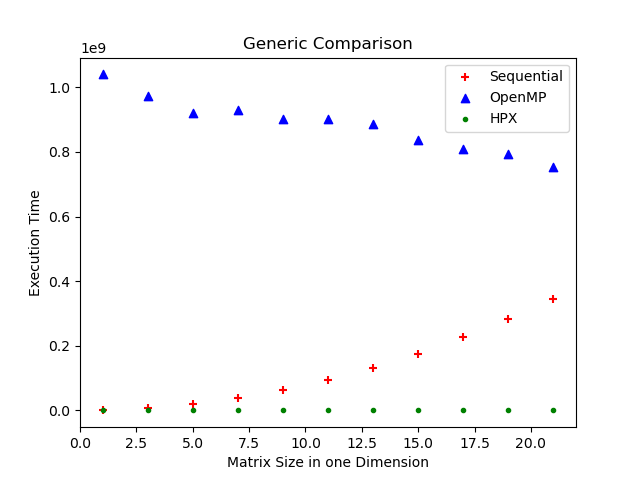
\includegraphics[width=0.45\textwidth]{figures/genericMatrix.png}
	\caption{Execution Times of Generic Algorithm Task Matrices of all Versions and only HPX(Environment 4, 12 Threads)}
	\label{fig:genMatrix}
\end{figure}

Figure \ref{fig:genMatrix} part a) shows the average execution time of 25 runs.
As already mentioned, the number of tasks are the same for all executions.
Increasing the matrix size increases the task size and overall workload as it can be seen by the sequential execution's curve.
The HPX execution time looks like to have a quite constant trend.
However, this is due to the graphical illustration.
Having only the HPX data points in part b) of figure \ref{fig:genMatrix} one can see that the execution time of HPX also increases.
The numbers are just so small that it cannot be seen in the scatter plot above.

OpenMP's curve decreases with an increasing task size, although the overall workload increases.
This behavior is quite strange as the number of tasks stays constant.
Running results of the same experiment with setting different amounts of threads are illustrated in figure \ref{fig:genMatrix_Threaded}.

\begin{figure}[h]
	\centering
	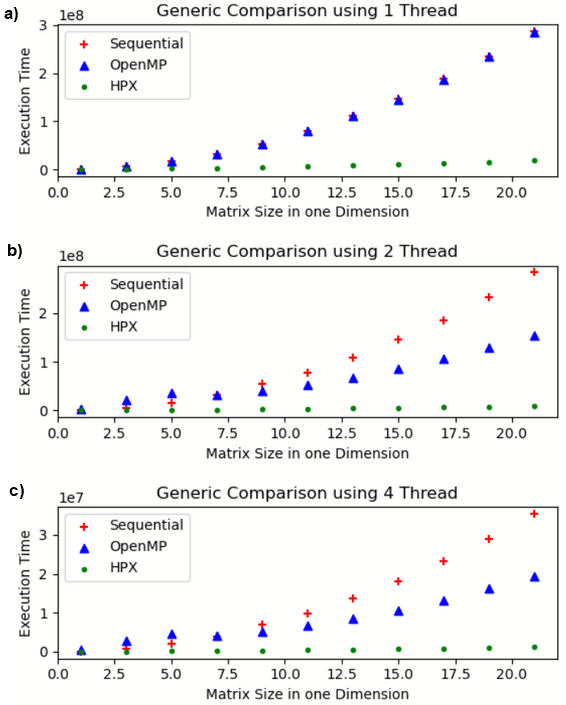
\includegraphics[width=0.45\textwidth]{figures/genericMatrix_Threaded.png}
	\caption{Execution Times of Generic Algorithm Task Matrices for different amount of threads a) = 1 b) = 2 c) = 4(Environment 4)}
	\label{fig:genMatrix_Threaded}
\end{figure}

Part a) shows results for \texttt{OMP\_NUM\_THREADS=1} and \texttt{--hpx:threads=1}.
OpenMP here behaves as expected.
Part b) shows the results for setting the used threads equal to 2 and c) for 4.
There is the possibility that OpenMP might have some problems with bigger amounts of threads for this algorithm.
At least in case the task size is rather small.
However, it is not possible yet to explain this behavior in detail.

\subsection{Generic Algorithm - Sanity Tests}
The last experiment of this section is a sanity test to test the behavior of the OpenMP and HPX implementations using one and two tasks in parallel.
It is expected that when executing the generic algorithm with a tasks size equal to the size of the array the execution time must be similar to the one of the sequential implementation.
The generic algorithm is given a task size equal to the size of the array and another one equal to half of the array size.
Therefore only one or two tasks are in use per turn.
Furthermore the final summation of all elements is exchanged in favor of the sequential version.
\begin{figure}[h]
	\centering
	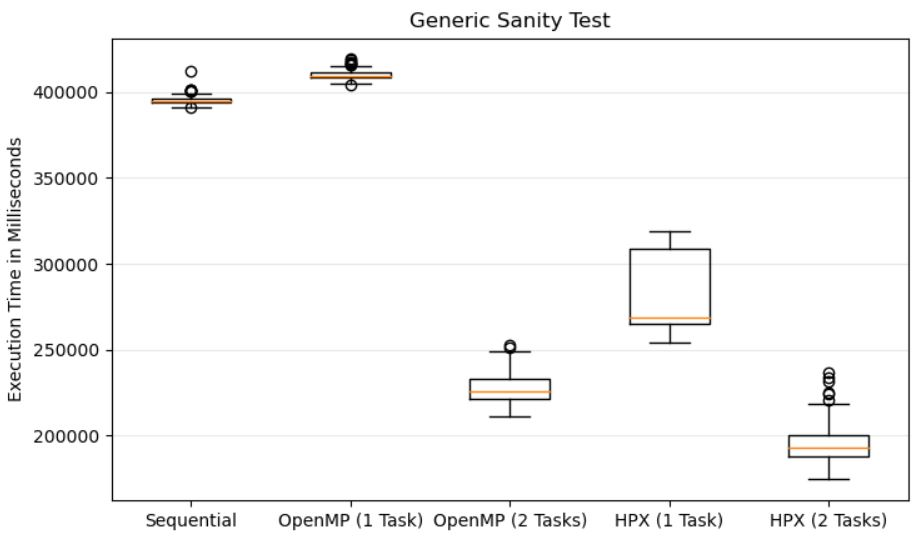
\includegraphics[width=0.45\textwidth]{figures/sanity.jpg}
	\caption{Sanity Tests for Generic Algorithm (Environment 3, 64 Threads)}
	\label{fig:sanity}
\end{figure}

Figure \ref{fig:sanity} shows the execution times for this experiment.
It can be seen that the OpenMP version using one tasks takes about the same time as the sequential version and using two tasks decreases the execution time significantly.
For the OpenMP implementation it is important to set the \texttt{OMP\_NUM\_THREADS} variable equal to the simultaneously used tasks.
Otherwise the OpenMP version takes longer than the sequential implementation.
These may be due to the fact that different cores may execute the code.
Doing so forces to use a different part of the CPU cache and nihilists the lines loaded before.

Important to notice is that the HPX implementation takes less time to execute the generic algorithm with one task.
This is also tested using \textit{system} and \textit{tcalloc} allocation options during build.
However both options result in no significant difference in execution time.


\section{Conclusion \& Future Work}



\bibliographystyle{unsrt}
\bibliography{paper}{}

\end{document}


% Maybe extensions
% compare with BOTS - fib / sort
% 